% Final §2 -- Business model and cloud vs on-premise cost (plan §7.1: 1.25 pages).
% Cost numbers: results/cost/model-summary.md via generated/numbers.tex; method: docs/COST.md.
\section{Business model and cost}\label{sec:business}

\paragraph{Customers, pricing and value.}
Organisers pay; participants never pay or install anything. We propose two plans: a free tier with
one open workshop at a time, and an organiser plan at \sd10 per organisation per month (\sd120 a
year) with any number of open workshops and co-organisers. The prototype does not enforce plan
limits. The first channel is NUS student organisations and units that run repeated workshops,
starting with the pilot organiser (\S\ref{sec:pilot}). The price is defensible if
$h \cdot w \cdot k \geq P$, where $h$ is the coordination time saved per multi-session event, $w$
the value of an organiser hour and $k$ the number of such events per organiser-year. The organiser
interviews give $h$ (median \InterviewHoursMedian{} hours per event) and the willingness to pay
(median price felt to be a bargain \InterviewWtpBargainMedian{}, getting expensive
\InterviewWtpExpensiveMedian{} \sd/month). The simulation in \S\ref{sec:mechanism} gives one
component of $h$: with per-session forms, \ReplayDupConfirmedPerSessionMean{} confirmed seats per
workshop end as duplicates that the organiser must chase, against \ReplayDupConfirmedUnifiedMean{}
with one queue.

\paragraph{Cost accounting in three layers.}
Cloud cost is computed as usage $\times$ unit price for the \CostPricesTotal{} billable dimensions the
stacks use in \code{ap-southeast-1}; \CostPricesVerified{} of the \CostPricesTotal{} unit prices were read from
the AWS Price List API on \CostPricingDate~\cite{aws-pricelist-bulk-api}. The layers are (1)~list
price, (2)~after the always-free allowances~\cite{aws-free-tier}, and (3)~after credits, which is
\usd0 while the account's credits last. Layer~3 is why billing tools show a net cost of zero; our
budget alarms therefore exclude credits, whose inclusion is the default~\cite{aws-budgets-costtypes}.
Until measured usage is priced (\CostMeasuredListUsd), usage per registration is modelled from the
design: \CostAssumeCommandsPerRegistration{} commands and \CostAssumeOffersPerRegistration{} offers
per registration, \CostAssumeReadsPerCommand{} API reads per command including polling, and
\CostAssumeMauPerRegistration{} Cognito monthly active users per registration (all assumptions are
listed in \code{results/cost/model-summary.md}).

\paragraph{On-premise reference.}
The on-premise build runs the same engine and single-page application (SPA) (\code{services/local}:
Docker Compose with PostgreSQL, Keycloak, Mailpit and nginx) on one mini-PC. Two views are priced:
\emph{increment only} (hardware amortised over \CostAmortisationYears{} years, electricity, a static
IP, e-mail at the same provider price, no labour) and \emph{fully amortised} (plus a business fibre
line, an off-site backup copy and operations labour, which is an assumption). Load, retention and
functionality are held equal; availability is not: one machine has no failover, whereas the cloud
services span several availability zones (AZs).

\begin{table}[t]
\centering
\begin{minipage}[c]{0.505\textwidth}\centering\footnotesize
\begin{tabular}{@{}r@{\hspace{6pt}}rrr@{\hspace{8pt}}rr@{}}
\toprule
 & \multicolumn{3}{c}{Cloud} & \multicolumn{2}{c@{}}{On-prem (\CostAmortisationYears-yr)}\\
\cmidrule(r{6pt}){2-4}\cmidrule(l){5-6}
Registrations & list & after free & after & increment & fully\\
per month & price & tier & credits & only & amortised\\
\midrule
1{,}000   & \CostTierOneKCloudListUsd & \CostTierOneKCloudAfterFreeUsd & \CostTierOneKCloudAfterCreditsUsd & \CostTierOneKOnpremIncrementThreeYearUsd & \CostTierOneKOnpremFullThreeYearUsd\\
10{,}000  & \CostTierTenKCloudListUsd & \CostTierTenKCloudAfterFreeUsd & \CostTierTenKCloudAfterCreditsUsd & \CostTierTenKOnpremIncrementThreeYearUsd & \CostTierTenKOnpremFullThreeYearUsd\\
100{,}000 & \CostTierHundredKCloudListUsd & \CostTierHundredKCloudAfterFreeUsd & \CostTierHundredKCloudAfterCreditsUsd & \CostTierHundredKOnpremIncrementThreeYearUsd & \CostTierHundredKOnpremFullThreeYearUsd\\
\midrule
\multicolumn{6}{@{}l@{}}{Cloud list price per 1{,}000 registrations: \CostUnitOneKCloudListUsd{} / \CostUnitTenKCloudListUsd{} / \CostUnitHundredKCloudListUsd}\\
\bottomrule
\end{tabular}
\end{minipage}\hfill
\begin{minipage}[c]{0.475\textwidth}
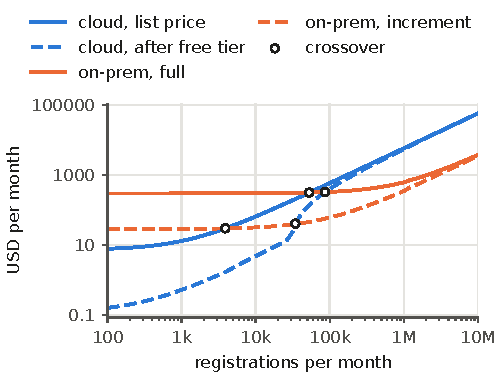
\includegraphics[width=\linewidth]{figures/generated/cost-crossover}
\end{minipage}
\caption{Monthly cost in \usd{} by load. Left: modelled cloud usage at list price, after the free
allowances and after credits, and the two on-prem views. Right: the same curves on a log--log scale
with the crossover points (the after-credits layer is 0 and not drawn). Sources:
\code{results/cost/model-summary.md}, \code{crossover-curve.csv}.}\label{tab:cost}
\end{table}

\paragraph{Result.}
At 1{,}000 registrations a month the cloud list price (\usd\CostTierOneKCloudListUsd) is mostly
fixed items, CloudWatch dashboard, metrics and alarms (\usd\CostSvcCloudWatchOneKListUsd) and
Cognito (\usd\CostSvcCognitoUserPoolsOneKListUsd), which the free allowances cover; what remains is
\usd\CostTierOneKCloudAfterFreeUsd{} (Table~\ref{tab:cost}). At 100{,}000 registrations Cognito
dominates the list price (\usd\CostSvcCognitoUserPoolsHundredKListUsd{} of
\usd\CostTierHundredKCloudListUsd). The fully amortised on-prem view is nearly flat because labour
(\usd\CostOnpremOneKFullLabourUsd) and the business line (\usd\CostOnpremOneKFullNetworkUsd) dominate
it. The cloud list price exceeds the increment-only view above \CostCrossoverListIncrementRegs{}
registrations a month and the fully amortised view above \CostCrossoverListFullRegs{}
(Table~\ref{tab:cost}, right; after the free tier: \CostCrossoverAfterFreeIncrementRegs{} and
\CostCrossoverAfterFreeFullRegs). Below the first crossover the cloud build is the cheaper option in
both views; up to the second it is cheaper than an on-prem service that pays for its own line and
operations. It costs nothing out of pocket while credits last and buys multi-AZ availability, which
a single volunteer-run machine gives up.
